\chapter{Level JSON Format Beschreibung}

\section{Präambel}
Die Auslieferung von Levels des Spiels wird auf Basis des verbreiteten JSON (JavaScript Object Notation) Formates und mittels Konventionen auf der Dateisystemhierarchie geschehen.
Die Gründe für die Verwendung von JSON sind
\begin{enumerate}[a)]
	\item Einfache Schreib- und Editierbarkeit
	\item Gute Les- und Nachvollziehbarkeit
	\item Geringerer Overhead gegenüber XML
	\item Unterstützung von Haus aus durch libgdx
	\item Gute Austausch- und Erweiterbarkeit gegenüber datenbank- oder codebasierten Herangehensweisen
\end{enumerate}
Dafür ist es zunächst jedoch erforderlich, dass die Struktur der letztendlich für den Aufbau eines Levels benötigten Daten, detailliert spezifiziert ist.
Im folgenden werden die einzelnen Attribute eines Levels und ihre Bedeutungen, sowie ihre Repräsentation in JSON beschrieben.

\section{Grundlegendes}
Im Folgenden wird stets davon ausgegangen, dass sich jegliche Dateisystem Pfadangaben relativ zu "`/assets"' beziehen, wobei als Wurzelverzeichnis das Android Projektverzeichnis angesehen wird.
Die Nutzung des "`asset"'-Ordners wird hierbei von libgdx vorgegeben.
Vergleiche hierzu den entsprechenden Artikel der Dokumentation \footnote{\url{https://github.com/libgdx/libgdx/wiki/File-handling\#android}}.
Zudem sei erwähnt, dass sich alle in JSON angegebenen Elemente, die von der Anwendung benutzt werden, im Namespace \strong{"'de.croggle"'} befinden.
Das heißt, dass sich in dem Wurzelobjekt jeder JSON Datei ein Objekt mit diesem Namen befindet.
Dies macht es sicherer, gegebenenfalls in Zukunft vom Nutzer angegebene Levels zu laden, auch wenn dies derzeit nicht als Funktion vorgesehen ist.
\begin{lstlisting}[language=json,caption={Standardinhalt jeder JSON Datei der Anwendung}]
{
	"de.croggle" : {
		...
	}
}
\end{lstlisting}
Die Spezifikation beschreibt lediglich die Elemente, die in Objekten verpflichtend vorhanden sein müssen.
Darüber hinausgehende Attribute werden von der Applikation ignoriert.
Sollten einzelne Elemente oder auch nur deren Inhalt als optional angesehen werden, ist dies entsprechend im Text ausgewiesen.

Da die Beschreibungen von Levels, ähnlich wie Quellcode, komplexe Sachverhalte im Lambda-Kalkül abbilden können, deren Wirkungsweise nicht direkt ersichtlich sein kann, sieht die Spezifikation der JSON Repräsentation Kommentarattribute vor.
Diese können und sollen verwendet werden, um besonders schwer nachzuvollziehende Stellen zu dokumentieren, aber auch, um einfach auf die Ideen und Zielsetzungen innerhalb eines bestimmten Levels hinzuweisen.
Solche Kommentarattribute werden durch das Präfix \strong{"'\_comment"'} markiert und eingeleitet.
Attributsnamen, die mit diesem beginnen sind dementsprechend reserviert.
Es muss zudem davon ausgegangen werden, dass sich an einer späteren Stelle der Entwicklung ein Mechanismus im Build System befindet, der die Kommentare vor der Auslieferung aus den JSON Dateien entfernt.

Da die Kommentare jeweils durch eine Zeichenkette im Namen eines Attributes eingeleitet werden und JSON keine Namen von Attributen in Listen (eingeleitet durch "'["') vorsieht, sind Kommentare nur in Objekten (eingeleitet durch "'\{"') zulässig.
Dies ist insofern keine Einschränkung, da Listen im Allgemeinen nur anonyme Instanzen von Elementen beinhalten, deren es für gewöhnlich keinerlei weitere Erklärungen bedarf.
Der Wert eines solchen Kommentarattributes kann einerseits aus einem einfachen Stringliteral (Zeichenkette) bestehen, wenn es sich um kurze, einzeilige Kommentare handelt.
Andererseits kann bei längeren Kommentaren auch eine Liste von Stringliteralen angegeben werden, wobei jedes Element auf eine neue Zeile geschrieben wird.
Damit wird der Einschränkung im JSON Format Rechnung getragen, dass es keine Möglichkeit gibt, sogenannte Multiline Strings anzugeben.
Zuletzt ermöglicht die Spezifikation auch mehrere Kommentarattribute innerhalb des gleichen Objektes.
Dafür wird den jeweiligen \strong{"'\_comment"'}-Attributnamen noch jeweils eine Ziffernfolge angehängt, welche von Null beginnend aufsteigt.
Dies ist nötig, da der JSON Standard keine gleichen Attributnamen innerhalb einunddesselben Objekts vorsieht.
Listing 4.2 verdeutlicht die Anwendung von Kommenatren in JSON Files.

\needspace{5cm}
\begin{lstlisting}[language=json,caption={Kommentare in einer JSON Datei}]
{
	"_comment" : "Dies ist ein kurzer Kommentar",
	"de.croggle" : {
		"_comment": [
			"Längere Kommentare, die ",
			"über mehrere Zeilen gehen, ",
			"werden mittels einer Liste repräsentiert"
		]
	},
	"_comment0" : "Mehrere Kommentare in ein und demselben Objekt...",
	"_comment1" : "... werden mittels aufsteigender Nummern als Postfix unterschieden"
}
\end{lstlisting}

\section{Levels}
Bisher sind folgende Leveltypen für das Spiel vorgesehen:
\begin{itemize}
	\item Multiple Choice Levels (MC)
	\item Färben und Einfügen (FE)
	\item Schrittanzahl (SA)
\end{itemize}
Um ein Level zur Laufzeit zu laden, müssen die folgenden Daten zur Verfügung stehen:
\begin{enumerate}[a)]
	\item Das Levelpaket, zu dem ein Level gehört
	\item Die Position des Levels innerhalb eines Levelpakets
	\item Eine Zeichenkette, die auf das Level einstimmt
	\item Eine (optionale) Animation zu Beginn eines Levels
	\item Eine optionale Anzahl Schritte, nach der die Simulation automatisch beendet wird
	\item Der Name eines Designthemas (es kann sich auch nur um den Pfad zu einem Hintergrundbild handeln)
	\item Ein Tipp, um das Level abzuschließen
	\item Den Typ eines Levels
	\item Konstellationen (Anfang, Ende, mögliche Antworten)
\end{enumerate}
Zur Angabe dieser Daten existiert zu jedem Level eine JSON Datei (Endung \strong{"'.json"'}), deren Name der auf zwei Stellen aufgefüllten Identifikationsnummer innerhalb eines Levelpakets entspricht.
Dies ermöglicht das schnelle Auflisten aller Levels eines Pakets, impliziert aber auch, dass ein Levelpaket höchstens 100 Level enthalten kann.
Zur Vermeidung von Namenskollisionen zwischen Levels verschiedener Pakete, erhält jedes Paket sein eigenes Unterverzeichnis.
Dazu jedoch mehr in Kapitel "'Levelpakete"'.
Innerhalb einer solchen JSON Datei existiert (im Applikationsnamensraum) eine Liste mit dem Namen \strong{"'levels"'}.
An dieser Stelle wäre auch ein einfaches Objekt möglich, welches direkt alle notwendigen Daten enthält.
Der gewählte Ansatz bietet allerdings die Vorteile, dass erstens direkt auf die Levels als solche zugegriffen werden kann, da keine Typprüfung stattfinden muss (\strong{"'levels"'} darf nur Levels enthalten).
Zweitens lassen sich gegebenenfalls alle Levels in dieser Liste zusammenlegen, was nur noch eine JSON Datei notwendig machen und somit Spielraum für Leistungsverbesserungen bieten würde.
Und drittens muss kein Name für die sonst eigentlich anonymen Levels angegeben werden.


Innerhalb dieses Grundgerüstes werden alle weiteren, notwendigen Daten spezifiziert.
Zuerst genannt sei hierbei die Beschreibung: Unter dem Attributsnamen \strong{"'description"'} wird hierbei die auf das Level einstimmende Zeichenkette abgelegt.
Unter dem Attribut \strong{"'design"'} ist, wie erwähnt, entweder der Name eines Designthemas oder der Name/Pfad zu einem alternativen Hintergrundbild in einer Zeichenkette gespeichert.
Bei einer leeren Zeichenkette wird das Standardthema des Levelpakets verwendet.
In einem Feld \strong{"'abort simulation after"'} kann optional die ganzzahlige Anzahl an Ausführungsschritten abgelegt werden, nach denen ein Level als beendet angesehen wird.
Positive Werte implizieren, dass im Anschluss das Level als erfolgreich abgschlossen gewertet werden soll.
Bei einem negativen Wert gilt das Level nach Ablauf der Schrittzahl als verloren.
Der Wert Null ("'0"') bedeutet hierbei, dass kein Abbruch geschieht, was dem voreingestellten Verhalten entspricht.
Das Attribut \strong{"'hints"'} bezeichnet eine Liste von Zeichenketten, die Pfade zu Hilfegrafiken angeben, die der Nutzer als Hilfestellung anzeigen lassen kann.
Im derzeitigen Entwurf ist nur ein einziger Tipp pro Level vorgesenen.
Orientiert an anderen Spielen auf dem Markt hält eine Liste allerdings die Möglichkeit offen, weitere Tipps pro Level hinzuzufügen, ohne dass die JSON Spezifikation geändert werden muss.
In diesem Falle würden die Tipps in der Reihenfolge aufgedeckt werden, in der sie in der Liste vorkommen.
Die Liste an sich kann allerdings auch leer bleiben.

Unter dem Namen \strong{"'type"'} muss eine Zeichenkette existieren, die einen der folgenden Werte enthalten muss:
\begin{itemize}
	\item multiple choice
	\item modification
	\item step count
\end{itemize}

Für jeden dieser Typen unterscheidet sich der Inhalt des letzten Attributs, dem \strong{"'data"'} Attribut.
Dieses enthält die für die einzelnen Typen unterschiedlichen Daten.
Diese werden im Folgenden spezifiziert.
Listing 4.3 beschreibt das benötigte Rahmenwerk für alle Levels.

\needspace{5cm}
\begin{lstlisting}[language=json,caption={JSON Leveldatei, z.B. json/00/00.json}]
{
	"de.croggle" : {
		"levels" : [
			{
				"type" : "...",
				"description" : "...",
				"design" : "...",
				"abort simulation after": "...",
				"hints" : [
					...
				],
				"data" : {
					...
				}
			}
		]
	}
}
\end{lstlisting}

\subsection{Darstellung von Lambda-Ausdrücken}
Alle Leveltypen haben gemein, dass sie an mindestens einer Stelle ein Spielfeld mit einem Alligatorausdruck anzeigen.
Daher wird zunächst auf die Darstellung eines solchen Spielfelds mit der sich darauf befindlichen Konstellation (dem Lambda-Term) in der JSON Levelbeschreibung eingegangen.
Diese Darstellung bildet das zu den Lambda-Termen gehörige Klassenmodell transparent ab.


Das heißt, dass Spielfelder (im Folgenden auch Boards genannt) eine Liste von Elementen, genauer gesagt von BoardObjects, als Attribut besitzen.
Von diesen BoardObjects existieren drei Typen, nämlich Ei, farbiger Alligator und alter Alligator.
Alle diese drei Objekttypen verfügen über eine Zeichenkette mit Namen \strong{"'type"'}.
Zusätzlich wird über den Wahrheitswert im Feld \strong{"'movable"'} festgelegt, ob der Nutzer das Objekt nachträglich bewegen darf.
Ob er es ganz vom Spielfeld entfernen darf, wird mit dem Feld \strong{"'removable"'} angegeben.

Das \strong{"'type"'}-Attribut, darf die folgenden Werte annehmen:
\begin{itemize}
	\item egg
	\item colored alligator
	\item aged alligator
\end{itemize}
Aus diesem Attribut wird der genaue Typ eines BoardObjects abgeleitet, aus dem die weiteren Attribute hervorgehen.
Diese sind im Folgenden beschrieben.

\subsubsection{Eier}
Objekte vom Typ \strong{"'egg"'} besitzen die folgenden Eigenschaften:
\begin{description}
	\item[color:] Eine Ganzzahl >= 0, die einer Farbe zugeordnet wird. Der Wert befindet sich zwischen 0 und 30. Negative Werte werden als "'keine Farbe/ungefärbt"' interpretiert.
	\item[recolorable:] Wahrheitswert, ob das Objekt vom Nutzer nachträglich manuell umgefärbt werden darf.
\end{description}

\subsubsection{Farbige Alligatoren}
Objekte vom Typ \strong{"'colored alligator"'} besitzen die folgenden Eigenschaften:
\begin{description}
	\item[color:] Eine Ganzzahl >= 0, die einer Farbe zugeordnet wird. Der Wert befindet sich zwischen 0 und 30. Negative Werte werden als "'keine Farbe/ungefärbt"' interpretiert.
	\item[recolorable:] Wahrheitswert, ob das Objekt vom Nutzer nachträglich manuell umgefärbt werden darf.
	\item[children:] Eine Liste von weiteren BoardObjects
\end{description}

\subsubsection{Alte Alligatoren}
Objekte vom Typ \strong{"'aged alligator"'} besitzen die folgenden Eigenschaften:
\begin{description}
	\item[children:] Eine Liste von weiteren BoardObjects
\end{description}

\needspace{5cm}
\begin{lstlisting}[language=json,caption={Ein einfaches Board mit allen existierenden BoardObjects}]
{
	"families" : [
		{
			"type" : "colored alligator",
			"movable" : false,
			"removable" : false,
			"color" : 0,
			"recolorable" : false,
			"children" : [
				{
					"type" : "aged alligator",
					"movable" : false,
					"removable" : false,
					"children" : [
						{
							"type" : "egg",
							"movable" : false,
							"removable" : false,
							"color" : 0,
							"recolorable" : false
						},
						{
							"type" : "egg",
							"movable" : false,
							"removable" : false,
							"color" : 0,
							"recolorable" : false
						}
					]
				},
				{
					"type" : "egg",
					"movable" : false,
					"removable" : false,
					"color" : 0,
					"recolorable" : false
				}
			]
		}
	]
}
\end{lstlisting}
	
\begin{figure}[h]
	\caption{Der durch das vorausgehende Listing dargestellte Alligatorausdruck}
	\begin{center}
		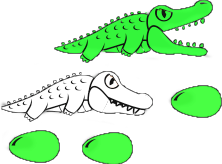
\includegraphics[width=0.3\textwidth]{../assets/lx.((x x) x).png}
	\end{center}
\end{figure}

\subsection{"'Multiple Choice"' Leveldaten}
Multiple Choice Levels benötigen eine Spielfeldkonstellation für die Ausgangsstellung und eine Liste mit möglichen Antwortoptionen, die auch als Spielfelder modelliert werden.
Hierbei wird bewusst keine feste Anzahl an Antworten festgelegt, auch wenn die Unterstützung durch das Programm nach der Implementierung nur bestimmte Anzahlen vorsieht.
Außerdem wird noch ein Index für die Konstellation benötigt, welche die Richtige ist.
Die Ausgangsstellung wird als Board in einem Feld mit Namen \strong{"'initial constellation"'} angegeben.
Die Liste mit Boards, die als mögliche Antworten dienen, heißt \strong{"'answers'"}.
Diese Liste muss mindestens ein Element enthalten.
Der Index der richtigen Antwort wird als Ganzzahl im Schlüssel \strong{"'correct answer"'} gespeichert.
Er bezieht sich auf die Position der gemeinten Konstellation in der \strong{"'answers"'} Liste, wobei ab Null angefangen wird zu indizieren.
Es ist jedoch zu beachten, dass die Reihenfolge der Elemente in der Liste keinen Einfluss auf deren Position in der dem Nutzer gezeigten Liste mit Antworten hat.
Diese wird nämlich randomisiert erstellt.

\needspace{5cm}
\begin{lstlisting}[language=json,caption={Grober Aufbau des data Attributs eines Multiple Choice Levels}]
"type" : "multiple choice",
"data" : {
	"initial constellation" : {
		...
	},
	"answers" : [
		...
	],
	"correct answer" : 0
}
\end{lstlisting}

\subsection{"'Färben und Einfügen"' Leveldaten}
Bei "'Färben und Einfügen"'-Levels werden nur die Ausgangskonstellation, die zu erreichende Endkonstellation und Listen mit für den Nutzer gesperrte Farben und Objekttypen als Angabe benötigt.
Die Ausgangskonstellation findet sich wie bei Multiple Choice Leveln im Feld \strong{"'initial constellation"'}, und wird mittels eines Board Objektes repräsentiert.
Die Endkonstellation kann über das Board-wertige Attribut \strong{"'objective"'} ausgelesen werden.
Gesperrte Farben werden durch eine Liste mit Ganzzahlen >= 0 dargestellt, die den Namen \strong{"'blocked colors"'} trägt.
Gesperrte Objekttypen können in einer Liste von Zeichenketten mit Namen \strong{"'blocked types"'} angegeben werden, wobei deren Werte den bekannten Typen aus der Dartellung von Lambda-Ausdrücken entspricht.
Diese Funktion ist vor allem für die Tutorial Levels vorgesehen, wenn das Platzieren von Eiern etc. verhindert werden soll.

\needspace{3cm}
\begin{lstlisting}[language=json,caption={Grober Aufbau des data Attributs eines "'Färben und Einfügen"' Levels}]
"type" : "modification",
"data" : {
	"initial constellation" : {
		...
	},
	"objective" : {
		...
	},
	"blocked colors" :  [
		...
	],
	"blocked types" : [
		...
	]
}
\end{lstlisting}

\subsection{"'Schrittanzahl"' Leveldaten}
In Levels, in denen die Schrittanzahl zum Gewinnen des Levels entscheidend ist, werden grundsätzlich die gleichen Daten im data Attribut bereitgestellt, wie schon für den Typ "'Färben und Einfügen"'.
Lediglich ist hier das Element \strong{"'objective"'} nicht mehr vonnöten.
Das Ziel wird stattdessen nur von dem ohnehin für jeden Leveltyp vorgesehenen Wert \strong{"'abort simulation after"'} außerhalb des data Attributs spezifiziert.

\begin{lstlisting}[language=json,caption={Grober Aufbau des data Attributs eines "'Schrittzahl"' Levels}]
"type" : "step count",
"data" : {
	"initial constellation" : {
		...
	},
	"blocked colors" :  [
		...
	],
	"blocked types" : [
		...
	]
}
\end{lstlisting}

\section{Levelpakete}
Levels werden durch sogenannte Pakete gruppiert.
Diese Pakete besitzen folgende Eigenschaften, die durch die Spezifikation repräsentiert werden müssen:
\begin{enumerate}[a)]
	\item Eine Position des Pakets, um die Reihenfolge der Pakete festzulegen
	\item Eine Verbindung zwischen dem Paket und den dazugehörigen Leveln
	\item Ein Name zur Bezeichnung des Pakets
	\item Eine kurze, optionale Beschreibung des Pakets
	\item Eine Grafik, die zum Thema des Pakets passt
	\item Ein Designthema, in dem das Paket und die enthaltenden Levels standardmäßig angezeigt werden.
	\item Eine Angabe zu etwaigen Animationen, die beim ersten Spielen des Pakets gezeigt wird.
	\item Abhängigkeiten, die zum Freischalten der Box erfüllt sein müssen
\end{enumerate}
Hierbei muss jedoch nicht allein auf JSON zurückgegriffen werden.
Auch Dateisysteminformationen können berücksichtigt werden.
Es muss lediglich bedacht werden, dass durch Festlegung von Konventionen keine zu starke Einschränkung passiert, sodass die Erweiterbarkeit nicht eingeschränkt wird.

Grundsätzlich existiert zu jedem Level unter json/levels/ ein Ordner mit der Position des Pakets in der Liste der Pakete.
Auch hier wird der Index als zweistellige Zahl mit den Ziffern 0 bis 9 dargestellt, was eine theroetische maximale Anzahl von 100 verschiedenen Levelpaketen erlaubt.
In jedem dieser Ordner befinden sich die zu dem Paket gehörenden Levels in jeweils einer eigenen JSON Datei, die nach dem in Abschnitt "'Levels"' beschriebenen Schema benannt sind.
Diese Maßnahmen decken bereits die ersten beiden Punkte, die für die Beschreibung eines Levelpakets nötig sind, ab.
Zusätzlich existiert in dem Paketordner eine weitere JSON Datei mit dem Namen \strong{"'package.json"'}.
Diese dient dazu, die restlichen der eben aufgelisteten Daten anzugeben.
Wie dies genau geschieht wird im Folgenden spezifiziert.
\newline
Wie bereits bei Levels geschieht die Definition eines Levels nicht über einen festen Namen im Namensbereich des Spiels.
Stattdessen wird ein anonymes Objekt in einer Liste verwendet.
Diese Liste heißt \strong{"'packages"'}.
Listing 4.8 verdeutlicht die Folgen dieses Sachverhalts.
Der Name eines Packages wird im Feld \strong{"'name"'} als Zeichenkette eingetragen.
Die Zeichenkette zur Beschreibung erfolgt wie bei Leveln im \strong{"'description"'} Attribut.
Mittels einer Zeichenkette \strong{"'banner"'} wird der Pfad zu einer für das Level stehenden Grafik spezifiziert.
Auch die Angaben von Designthema und Animation beim ersten Betreten werden durch Pfade in Zeichenketten angegeben.
Für ersteres heißt diese \strong{"'design"'}, für zweiteres \strong{"'animation"'}.
Die Paketdesigns können von Levels mittels des dazu vorgesehenen \strong{"'design"'} Attributes überschrieben werden.
Da die Beschreibung von Abhängigkeiten eine größere Komplexität aufweist, ist ihr im folgenden eine Untersektion gewidmet.
Grundsätzlich werden sie in einer Liste mit dem Namen \strong{"'dependencies"'} definiert.
Das folgende Listing veranschaulicht all diese Spezifikationen.

\needspace{5cm}
\begin{lstlisting}[language=json,caption={Standardinhalt der Definition eines Levels}]
{
	"de.croggle" : {
		"packages" : [
			{
				"_comment" : "Die Definition eines Paketes erfolgt hier",
				"name" : "...",
				"decription" : "...",
				"banner" : "...",
				"design" : "...",
				"animation" : "...",
				"dependencies" : [
					...
				]
			}
		]
	}
}
\end{lstlisting}

\subsection{Abhängigkeiten}
Zum Freischalten eines Levelpakets können folgende Typen von Abhängigkeiten vorgegeben sein:
\begin{itemize}
	\item Vorhergehendes Levelpaket zu einem gewissen Grad abgeschlossen
\end{itemize}

Abhängigkeiten werden grundsätzlich durch Objekte abgebildet, die mindestens das Attribut \strong{"'type"'} aufweisen, mit dem weitere Felder - je nach Typ - eingeführt werden können.
Folgende Typen sind bisher definiert:
\begin{description}
	\item[packageprogress:] Wie weit ein bestimmtes anderes Levelpaket abgeschlossen sein muss, damit das Paket freigeschaltet ist.
\end{description}
Im Folgenden sind den jeweiligen Typen Abschnitte gewidmet, in denen weitere Attribute, die durch die Angabe eines Typseingeführt werden, erklärt sind.

\subsubsection{Paketfortschritt: "'packageprogress"'}
Für die Angabe eines mindestens benötigten Fortschritts eines Pakets werden Felder für das gemeinte Paket und für den Fortschritt benötigt.
Für Ersteres heißt dieses \strong{"'package"'} und beinhaltet eine Ganzzahl größer Null und kleiner 100.
Zweiteres findet sich im Feld \strong{"'progress"'}, welches auch eine Ganzzahl enthält, die den Fortschritt in Prozent darstellt.
Der Wert befindet sich also zwischen einschließlich 0 und 100.
Null Prozent heißt hierbei lediglich, dass das Level freigeschaltet sein muss. 
Das Gesperrtsein eines Pakets kann also keine Abhängigkeit sein.
Bei hundert Prozent müssen alle Levels erfolgreich abgeschlossen worden sein, die zu dem angegebenen Paket gehören.
Das folgende Listing fasst dies noch einmal zusammen.

\needspace{5cm}
\begin{lstlisting}[language=json,caption={Beispielhafte Definition einer Abhängigkeit vom Typ "'boxprogress"'}]
{
	"type" : "packageprogress",
	"_comment" : "Alle Levels des ersten Pakets müssen zum Freischalten erfolgreich abgeschlossen worden sein",
	"package" : 0,
	"progress" : 100
}
\end{lstlisting}

\section{Zusammenfassung}
\subsection{Dateisystemstruktur}
Ordnerübersicht zur Levelspezifikation
\dirtree{%
.1 assets/.
	.2 json/.
		.3 levels/.
			.4 00/.
				.5 00.json.
				.5 01.json.
				.5 \ldots{}.
				.5 package.json.
			.4 01/.
				.5 \ldots{}.
}

\subsection{Inhalte einer "`package.json"' Datei}
\dirtree{%
.1 \strong{"'de{.}croggle"'} : Object - Namensraum.
	.2 \strong{"'packages"'} : List - Liste mit Repräsentationen von Paketen{.} Gewöhnlich nur ein Paket.
		.3 : Object - Das zur Datei gehörende Paket als JSON Objekt.
			.4 \strong{"'name"'} : String - Der Anzeigename des Levelpakets.
			.4 \strong{"'description"'} : String - Eine Zeichenkette zur Beschreibung des Pakets.
			.4 \strong{"'banner"'} : String - Pfad zu einer Bilddatei, die als Banner für ein Levelpaket fungiert.
			.4 \strong{"'design"'} : String - Pfad zu einem Design, das auf alle Levels eines Pakets angewendet wird.
			.4 \strong{"'animation"'} : String - Pfad zu einer Animation, die vor dem ersten Betreten des Levels abgespielt wird.
			.4 \strong{"'dependencies"'} : List - Die Liste mit Abhängigkeiten.
				.5 \strong{"'type"'} : String - Der Typ einer Abhängigkeit.
				.5 Weitere Elemente für "'packageprogress"' Abhängigkeiten.
					.6 \strong{"'package"'} : unsigned Integer - Die Identifikationsnummer eines Pakets als Abhängigkeit.
					.6 \strong{"'progress"'} : unsigned Integer - Prozentzahl, zu der ein Paket als Abhängigkeit abgeschlossen sein muss.
}

\subsection{Inhalte einer Level JSON Datei}
\subsubsection{Rahmenwerk}
\dirtree{%
.1 \strong{"'de{.}croggle"'} : Object - Namensraum.
	.2 \strong{"'levels"'} : List - Liste mit Levelobjekten{.} Gewöhnlich nur ein Paket.
		.3 : Object - Darstellung einzelner Levels.
			.4 \strong{"'type"'} : String - Typ eines Levels.
			.4 \strong{"'description"'} : String - Beschreibung zu einem Level.
			.4 \strong{"'design"'} : String - Pfad zu einem Leveldesign.
			.4 \strong{"'abort simulation after"'} : Integer - Nach wie vielen Schritten ein Level gewonnen (positiv) oder verloren (negativ) ist.
			.4 \strong{"'hints"'} : List - Strings mit Pfaden zu Hilfegrafiken.
			.4 \strong{"'data"'} (multiple choice) : Object - Spezielle Daten für die einzelnen Leveltypen.
				.5 Daten für MC Levels
					.6 \strong{"'initial"'} : Object - Board Objekt der An\-fangs\-kon\-stel\-la\-tion.
					.6 \strong{"'answers"'} : List - Liste mit Board Objekten der möglichen Antworten.
					.6 \strong{"'correct answer"'} : unsigned Integer - Der Index der richtigen Antwort zur Fragestellung.
				.5 Daten für FE Levels.
					.6 \strong{"'initial constellation"'} : Object - Board Objekt der An\-fangs\-kon\-stel\-la\-tion.
					.6 \strong{"'objective"'} : Object - Board Objekt der zu erreichenden Konstellation.
					.6 \strong{"'blocked colors"'} : List - Liste mit Integer Werten, die blockierte Farben beschreiben.
					.6 \strong{"'blocked types"'} : List - String Liste mit Namen von Elementtypen, die im Level nicht platzierbar sind (egg, colored alligator, aged alligator).
				.5 Daten für SA Levels.
					.6 \strong{"'initial constellation"'} : Object - Board Objekt der Anfangskonstellation.
					.6 \strong{"'blocked colors"'} : List - Liste mit Integer Werten, die blockierte Farben beschreiben.
					.6 \strong{"'blocked types"'} : List - String Liste mit Namen von Elementtypen, die im Level nicht platzierbar sind (egg, colored alligator, aged alligator).
}

\subsubsection{Alligator-Baumstruktur}
\dirtree{%
.1 : Board - Objekt, das ein Spielfeld mit einer Konstellation modelliert.
	.2 \strong{"'families"'} : List - Eine Liste mit sogenannten "'BoardObjects"'.
		.3 BoardObject Objekte - Objekte, die Teil einer Konstellation auf dem Spielfeld sind.
			.4 \strong{"'type"'} : String - Der genaue Typ des vorliegenden BoardObjects{.} Die Unterscheidungen der Typen werden im Folgenden erläutert.
			.4 \strong{"'movable"'} : Bool - Ob das Objekt nachträglich vom Nutzer bewegt werden kann.
			.4 \strong{"'removable"'} : Bool - Ob das Objekt nachträglich vom Nutzer vom Board entfernt werden kann.
			.4 Die drei möglichen Typen von BoardObjects sind "'egg"', "'colored alligator"' und "'aged alligator"'.
				.5 Typ \strong{"'egg"'}.
					.6 \strong{"'color"'} : Integer - Die Identifikationsnummer der Farbe, die das Ei haben soll.
					.6 \strong{"'recolorable"'} : Bool - Ob das Objekt nachträglich vom Nutzer umgefärbt werden kann.
				.5 Typ \strong{"'colored alligator"'}.
					.6 \strong{"'color"'} : Integer - Die Identifikationsnummer der Farbe, die der Alligator haben soll.
					.6 \strong{"'recolorable"'} : Bool - Ob der Alligator nachträglich vom Nutzer umgefärbt werden kann.
					.6 \strong{"'children"'} : List - Eine Liste mit weiteren BoardObjects (Eier, Alligatoren\ldots{}), wie sie in diesem Listing beschrieben sind.
				.5 Typ \strong{"'aged alligator"'}.
					.6 \strong{"'children"'} : List - Eine Liste mit weiteren BoardObjects (Eier, Alligatoren\ldots{}), wie sie in diesem Listing beschrieben sind.
}
